\documentclass[12pt]{article}
\usepackage[top=1in, bottom=1in, left=1in, right=1in]{geometry}
%\usepackage[margin=1in]{geometry}
\usepackage[onehalfspacing]{setspace}
%\usepackage[doublespacing]{setspace}
\usepackage{amsmath, amssymb, amsthm}
\usepackage{enumerate, enumitem}
\usepackage{fancyhdr, graphicx, proof, comment, multicol}
\usepackage[none]{hyphenat} % This command prevents hyphenation of words
\binoppenalty=\maxdimen % This command and the next prevent in-line equation breaks
\relpenalty=\maxdimen
%    Good website with common symbols
% http://www.artofproblemsolving.com/wiki/index.php/LaTeX%3ASymbols
%    How to change enumeration using enumitem package
% http://tex.stackexchange.com/questions/129951/enumerate-tag-using-the-alphabet-instead-of-numbers
%    Quick post on headers
% http://timmurphy.org/2010/08/07/headers-and-footers-in-latex-using-fancyhdr/
%    Info on alignat
% http://tex.stackexchange.com/questions/229799/align-words-next-to-the-numbering
% http://tex.stackexchange.com/questions/43102/how-to-subtract-two-equations
%    Text align left-center-right
% http://tex.stackexchange.com/questions/55472/how-to-make-text-aligned-left-center-right-in-the-same-line
\usepackage{microtype} % Modifies spacing between letters and words
\usepackage{mathpazo} % Modifies font. Optional package.
\usepackage{mdframed} % Required for boxed problems.
\usepackage{parskip} % Left justifies new paragraphs.
\linespread{1.1} 


%figure support
\usepackage{import}
\usepackage{xifthen}
\pdfminorversion=7
\usepackage{pdfpages}
\usepackage{transparent}
\newcommand{\incfig}[1]{%
	\def\svgwidth{\columnwidth}
	\import{./figures/}{#1.pdf_tex}
}
\graphicspath{ {./figures/} }
\pdfsuppresswarningpagegroup=1

\newenvironment{problem}[1]
{\begin{mdframed}[linewidth=0.8pt]
        \textsc{Problem #1:}

}
    {\end{mdframed}}

\newenvironment{solution}
    {\textsc{Solution:}\\}
    {\newpage}% puts a new page after the solution
    
\newenvironment{statement}[1]
{\begin{mdframed}[linewidth=0.6pt]
        \textsc{Statement #1:}

}
    {\end{mdframed}}

%\newenvironment{prf}
 %   {\textsc{Proof:}\\}
 %   {\newpage}% puts a new page after the solution

\begin{document}
% This is the Header
% Make sure you update this information!!!!
\noindent
\textbf{CIS4367.01} \hfill \textbf{Brandon Thompson} \\
\normalsize Prof. Elibol \hfill Due Date: 2/5/20 \\

% This is where you name your homework
\begin{center}
\textbf{Homework 5}
\end{center}
	
	\begin{problem}{\#3.1}
		Explain the suitability or unsuitability of the following passwords:
		\begin{enumerate}[label=\alph*]
			\item qwerty
			\item Einstein
			\item wysiwyg (for ''what you see is what you get'')
			\item drowssap
			\item KVK919
			\item Florida
			\item *laptop\_admin\#
			\item cr\@zyp@ss
		\end{enumerate}
	\end{problem}
	\begin{solution}
		\begin{enumerate}[label=\alph*]
			\item All lowercase letters and they are consecutive on the
				keyboard. Unsuitable.
			\item No numbers, and password is a name, and thus is easily guessable.
				Unsuitable.
			\item Hard to guess phrase, more than 6 characters. Suitable.
			\item is the phrase 'password' backwards. Unsuitable.
			\item No special characters, fewer than 8 characters. Unsuitable.
			\item No special characters or numbers, password is a name and this is
				easily guessable. Unsuitable.
			\item Despite special characters in the front and back the majority is
				a common phrase that would be guessed. Unsuitable.
			\item More than 6 characters, includes special character. Suitable.
		\end{enumerate}
	\end{solution}


	\begin{problem}{\#3.2}
		An early attempt to force users to use less predictable passwords involved
		computer- supplied passwords. The passwords were eight characters long and
		were taken from the character set consisting of lowercase letters and digits.
		They were generated by a pseudorandom number generator with $2^{15}$ possible
		starting values. Using the technology of the time, the time required to
		search through all character strings of length 8 from a 36-character alphabet
		was 112 years. Unfortunately, this is not a true reflection of the actual
		security of the system. Explain the problem.
	\end{problem}
	\begin{solution}
		The number of possible strings that can be made from using 36 character with
		a length of 8 characters is $36^8 \approx 2^{41}$, but a pseudorandom number
		generator only has $2^{15}$ possible starting values. So you only need to check
		$2^{15}$ passwords.
	\end{solution}
	

	\begin{problem}{\#3.3}
		Assume that passwords are selected from four-character combinations of 26
		alphabetic characters. Assume that an adversary is able to attempt passwords
		at a rate of one per second.
		\begin{enumerate}[label=\alph*]
			\item Assuming no feedback to the adversary until each attempt has
				been completed, what is the expected time to discover the
				correct password?
			\item Assuming feedback to the adversary flagging an error as each
				incorrect character is entered, what is the expected time
				to discover the correct password? 
		\end{enumerate}
	\end{problem}
	\begin{solution}
		\begin{enumerate}[label=\alph*]
			\item Number of possible passwords $26^4 = 456976$, worst case check.\\
				Average amount of attempts is half the worst case.
				$\dfrac{26^4}{2}=228488$ attempts, or 228488 seconds.\\
				Number of seconds in a day is $60 \times 60\times 24 =86400$\\
				$\dfrac{228488}{86400} = 2.644$ days or $63.456$ hours to find the
				correct password.
			\item If user gets feedback with each character then the number of checks is
				$26 \times 4 = 104$ for the worst case. Then the average case is
				$\frac{104}{2}= 52$ checks or 52 seconds to find the correct password.
		\end{enumerate}
	\end{solution}


	\begin{problem}{\#3.6}
		Assume that passwords are limited to the use of the 95 printable ASCII characters
		and that all passwords are 10 characters in length. Assume a password cracker
		with an encryption rate of 6.4 million encryptions per second. How long will
		it take to test exhaustively all possible passwords on a UNIX system?
	\end{problem}
	\begin{solution}
		The number of possible password combinations from 95 characters with a length of 10
		is $95^{10} \approx 6\times 10^{19}$. The encryption rate is 6.4 million per second,
		or $6\times 10^6$ passwords per second.\\
		Then the total time to find all passwords on a UNIX system is:\\
		\\
		\[	
		\dfrac{6\times 10^{19} \text{\ passwords}}{6\times 10^6 \text{\ passwords/second}}
		= 9.4\times 10^{12} \text{\ seconds}
	.\]
		\\
		\\
		Seconds in a year is : $60 \times 60\times 24\times 365 =31536000 $ seconds
		$9.4\times 10^{12}\times \dfrac{1}{31536000} = $\\ 298072 years to test all possible passwords.
	\end{solution}


	\begin{problem}{\#3.7}
		Because of the known risks of the UNIX password system, the SunOS-4.0
		documentation recommends that the password file be removed and replaced with
		a publicly readable file called /etc/publickey. An entry in the file for user
		A consists of a user's identifier $ID_A$, the user's public key,
		$PU_a$, and the corresponding private key $PR_a$.

		This private key is encrypted using DES with a key derived from the user's
		login password $P_a$. When A logs in, the system decrypts $E\left( P_a, PR_a \right) $ 
		to obtain $PR_a$.
		\begin{enumerate}[label=\alph*]
			\item The system then verifies that $P_a$ was correctly supplied. How?
			\item How can an opponent attack this system?
		\end{enumerate}
	\end{problem}
	\begin{solution}
		The private and public key are inverse's, to validate $P_a$, the value of $PR_a$
		can be verified by encrypting the public key with an arbitrary number  $X$.
		Decrypt the encrypted value with $PR_a$.\\
		 \[
			 X = D\left( PR_a, E\left( PU_a,X \right)  \right) 
		.\] 
	\end{solution}


	\begin{problem}{\#3.8}
		It was stated that the inclusion of the salt in the UNIX password scheme
		increases the difficulty of guessing by a factor of 4096. But the salt is
		stored in plaintext in the same entry as the corresponding ciphertext
		password. Therefore, those two characters are known to the attacker and
		need not be guessed. Why is it asserted that the salt increases security? 
	\end{problem}
	\begin{solution}
		Salt serves three purposes:
		\begin{itemize}
			\item Prevents duplicate passwords from being visible in the password
				file. Even if two users choose the same password, they receive
				different salt values. So the hashed value of the passwords
				will be different.
			\item Increases difficulty of offline dictionary attacks. IF salt
				length is $b$ bits, the number of possible passwords is increased
				by $2^b$. Making it harder to guess a password.
			\item Makes it almost impossible to find out whether a person with passwords
				on two or more systems has used the same password on all of them.
		\end{itemize}
	\end{solution}


	\begin{problem}{\#3.9}
		Assuming that you have successfully answered the preceding problem and
		understand the significance of the salt, here is another question.
		Wouldn't it be possible to thwart completely all password crackers by
		dramatically increasing the salt size to, say, 24 or 48 bits?
	\end{problem}
	\begin{solution}
		No, protecting from password crackers depends on the user population.
		The password is generated with the original user entered password, a random
		salt, and a hash function.\\
		Increasing the salt size will stop multiple users from having the same
		salt value. If multiple users have the same salt value then the attacker
		needs to perform multiple encryptions per user password.
	\end{solution}


	\begin{problem}{\#3.11}
		For the biometric authentication protocols illustrated in Figure 3.12,
		note that the biometric capture device is authenticated in the case of
		a static biometric but not authenticated for a dynamic biometric.
		Explain why authentication is useful in the case of a stable biometric
		but not needed in the case of a dynamic biometric.
	\end{problem}
	\begin{figure}[ht!]
		\centering
		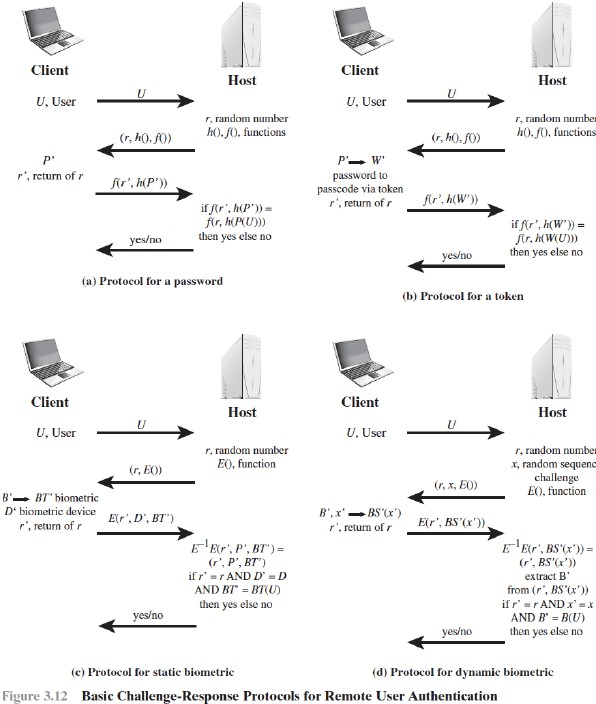
\includegraphics[width=0.8\textwidth]{fig3_12.jpg}
		\label{fig:3_12}
	\end{figure}
	\begin{solution}
		In dynamic biometric authentication, a random number $r$, and a random sequence $x$
		are used as a challenge. Because of the randomness in these numbers there is no need
		to have another layer of authentication.
	\end{solution}
\end{document}
